\documentclass[11pt,a4paper]{article}
\usepackage[utf8]{inputenc}
\usepackage[german]{babel}
\usepackage[T1]{fontenc}
\usepackage{amsmath}
\usepackage{amsfonts}
\usepackage{amssymb}
\usepackage{graphicx}
\usepackage[margin=1.25cm]{geometry} % Puts the same margin on all borders of the document

% Packages

\usepackage{hyperref} % Generate hyperlinks to referenced items
\usepackage{adjustbox} % Used to change parameters in \includegraphics[scale=•]{•}
\usepackage{enumitem} % Provides several options for lists
\usepackage{verbatim} % Package to use \begin{comment}
\usepackage{pdfpages} % Used to import PDF pages
\usepackage{multirow} % Allows us to have a single cell in a table span multiple rows
\usepackage{makecell} % Allows us to format multiple lines in a single cell
\usepackage{minted} % Used to syntax highlight code
\usepackage{xcolor}  % Gives access to coloring text
\usepackage{longtable} % Allows us to create a table over multiple pages
\usepackage{float} % Improved placement of floating items
\usepackage{pdfpages} % Used to import pdf pages
\usepackage{booktabs} % Used for horizontal lines instead of \hline



% Settings

\graphicspath{{./files/}} % Sets path for files to the files folder in the same directory

\hypersetup{
    colorlinks=false, %set true if you want colored links
    linktoc=all,     %set to all if you want both sections and subsections linked
    linkcolor=blue,  %choose some color if you want links to stand out
}

\begin{document}

\begin{center}
{\huge \textbf{Klausurblatt AfSE WiSe 19/20 | Skript: M. Otto}}\\
\end{center}


{\Large \textbf{Definitionen / Wissen}} 



\begin{itemize}

\item \textbf{Chomsky Hierarchie}



\begin{longtable}[h]{|p{4cm} | p{6cm} | p{7cm}|}

\hline
\textbf{Typ} & \textbf{Produktionen} & \textbf{Akzeptor} \\ \hline

Typ 0 - Allgemein & \makecell[l]{$\bullet$ beliebige Produktionen} &
\makecell[l]{$\bullet$ (D)TM akzeptiert nur teilweise \\ $\bullet$ (D)TM entscheidet nur teilweise \\ 
$\bullet$ rekursiv aufzählbar \\ $\bullet$ teilweise entscheidbar} \\ \hline

Typ 1 - Kontextsensitiv & \makecell[l]{$\bullet$ nur harmlose $\epsilon$-Produktionen \\ 
$\rightarrow$ $X_0 \rightarrow \epsilon$ \\
$\rightarrow$ $X_0$  nur als Startsymbol \\ $\rightarrow$ $X_0$ also nie auf rechter Seite \\
$\bullet$ Produktionen nicht verkürzend \\
$\rightarrow$ $\alpha \rightarrow \beta$ und $|\beta| \geq |\alpha|$} &
\makecell[l]{$\bullet$ (D)TM akzeptiert \\ $\bullet$ (D)TM entscheidet \\
$\bullet$ rekursiv aufzählbar und entscheidbar} \\ \hline


Typ 2 - Kontextfrei & \makecell[l]{$\bullet$ Linke Seite nur eine Variable \\ $\bullet$ X $\rightarrow$ v \\ $\bullet$ CNF möglich} &
\makecell[l]{$\bullet$ PDA akzeptiert \\ $\bullet$ CYK entscheidet \\ $\bullet$ rekursiv aufzählbar und entscheidbar} \\ \hline

Typ 3 - Regulär &  \makecell[l]{$\bullet$ Alle Produktionen rechtslinear \\
$\bullet$ X $\rightarrow \epsilon$, X $\rightarrow$ a, X $\rightarrow$ aY \\
$\bullet$ falls Variable, dann ganz rechts} &
\makecell[l]{$\bullet$ NFA akzeptiert \\ $\bullet$ DFA entscheidet \\$\bullet$ rekursiv aufzählbar und entscheidbar} \\ \hline

\end{longtable}

\item[]
	\begin{center}
	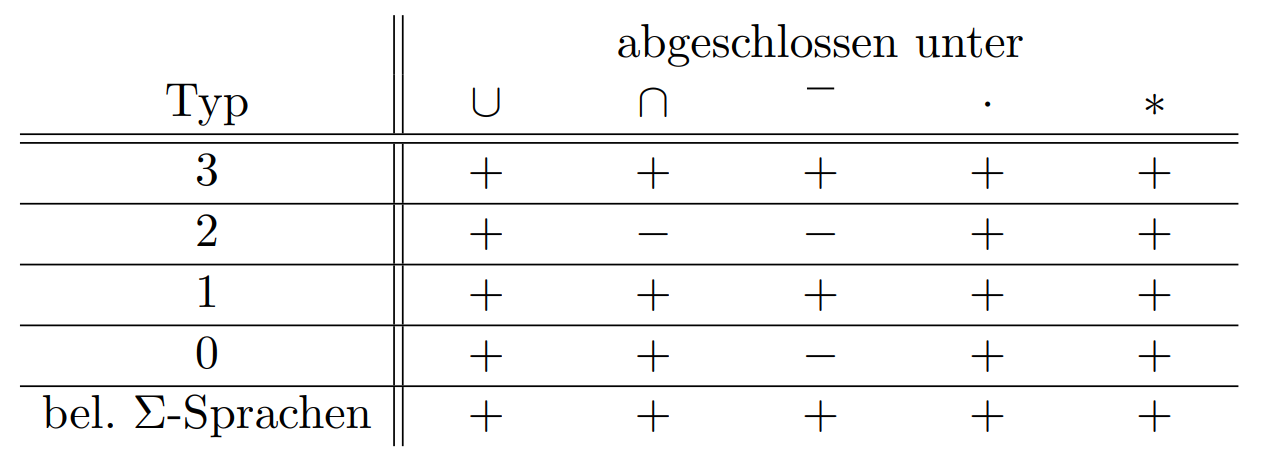
\includegraphics[width=14cm]{abschlussgrammatiken}
	\end{center}
	
\item \textbf{Sprachen im Niveau der Chomsky-Hierarchie}
	\begin{itemize}
	
	\item Sprache ($L \subseteq \Sigma^*$)	vom selben Typ wie Grammatik G, falls es Grammatik G gibt mit $L = L(G)$
	\item $L_{Typ3} \subsetneq L_{Typ2} \subsetneq L_{Typ1} \subsetneq L_{Typ0} \subsetneq \Sigma-Sprachen$
	\item $\subsetneq$ Echte Teilmenge
	
	\end{itemize}
	
\item \textbf{Grammatik-Tricks:}
	\begin{itemize}
	\item $X_0$: Neuer Startpunkt | $X_{0,1}:$ Startpunkt erste Grammatik
	\item Vereinigung: $X_0 \rightarrow X_{0,1} | X_{0,2}$
	\item Konkatenation: $X_0 \rightarrow X_{0,1} X_{0,2}$
	\item Stern-Bildung: $X_0 \rightarrow \epsilon|X_{0,1}X_0$ 
	\end{itemize}
	
\pagebreak	
	
\item {\large \textbf{Definitionen}}
	\begin{itemize}
	\item \textbf{Grammatik} $G = (\Sigma, V, P, S)$
		\begin{itemize}
		\item[$\rightarrow$] Terminalalphabet $\Sigma$, Variablen $V$, Produktionen $P$, Startsymbol $S$
		\end{itemize}
	\item \textbf{DFA/NFA} $A= (\Sigma, Q, q_0, \Delta/\delta, A)$
		\begin{itemize}
		\item[$\rightarrow$] Eingabealphabet $\Sigma$, Zustandsmenge $Q$, Startzustand $q_0$
		\item[$\rightarrow$] Übergangsrelation/-funktion $\Delta/\delta$, Akzeptierende Endzustände $A$
		\item[$\rightarrow$] $\Delta = Q~x~\Sigma~x~Q$ (Von q mit x nach q')
		\end{itemize}
		
	\item \textbf{PDA} $P = (\Sigma, \Gamma, Q, q_0, A, \Delta, \#)$
		\begin{itemize}
		\item[$\rightarrow$] Eingabealphabet $\Sigma$, Kelleralphabet $\Gamma$, Zustandsmenge $Q$, Startzustand $q_0$
		\item[$\rightarrow$] Akzeptierende Endzustände $A$, Übergangsrelation $\Delta$, Anfangs-Kellersymbol $\#$
		\item[$\rightarrow$] $\Delta = Q~x~\Gamma~x~(\Sigma \cup \{\epsilon\})~x~\Gamma^*~x~Q$
		\item[$\rightarrow$] (Von q, KellerPop, Lesenzeichen, KellerPush, nach q')
		\end{itemize}
		
	\item \textbf{Turingmaschine} $M = (\Sigma, Q, q_0, \delta, q+, q-)$
		\begin{itemize}
		\item[$\rightarrow$] Bandalphabet $\Sigma$, Zustandsmenge $Q$, Startzustand $q_0$
		\item[$\rightarrow$] Übergangsrelation $\delta$, akzeptierender Endzustand $q+$, verwerfender Endzustand $q-$
		\item[$\rightarrow$] $\delta = Q~x~(\Sigma \cup \{\square\}) \rightarrow (\Sigma \cup \{\square\})~x~\{<,o,>\}~x~Q$
		\item[$\rightarrow$] Von q, Lese vom Band $\rightarrow$ schreibe aufs Band, Bewege, nach q'
		\end{itemize}
	
	\end{itemize}
	
	
\item {\large \textbf{Beweis-Tipps}}
	\begin{itemize}
	
	\item \textbf{Mengenverhältnisse ($A \subseteq B$)}
		\begin{itemize}
		\item Am Besten über einzelne Elemente der Menge zeigen ($x \in A$)
		\item Zeigen, von welcher Menge x Element ist
		\item Danach Schluss darauf, dass es auch von anderer Seite Element ist
		\end{itemize}		
		
	
	\item \textbf{L(G) = L}
		\begin{itemize}
		\item $\supseteq$: Jedes w aus L ist in G $\rightarrow$ Induktion über die Wortlänge
		\item $\subseteq$: Jedes ableitbare Wort von G ist in L $\rightarrow$ Induktion über die Anzahl an Ableitungsschritten
		\end{itemize}
	
	\item \textbf{Beweise der Art $L_1 \cup L_2 = L \setminus ...$}
		\begin{itemize}
		\item Untersuchen, ob $\epsilon$ nur in einer Menge vorkommt (Widerlegbarkeit mit Gegenbeispiel)
		\end{itemize}
		
	\item \textbf{Gegenbeweis der Allaussage $\forall n \in \mathbb{N} A(n)$}
		\begin{itemize}
		\item Zeige, durch Gegenbeispiel $\exists n \in \mathbb{N} \lnot A(n)$
		\end{itemize}
		
	\item \textbf{Induktion über Wortlänge}
		\begin{itemize}
		\item Induktionshypothese IH | Induktionsanfang IA | Induktionsschritt IS
		\item IH: Aussage gilt für Wörter der Länge n
		\item IA: Zeige für Länge n = 0, also $\epsilon$
		\item IS: Wort der Länge n + 1 auf Länge n zurück führen
		\end{itemize}		
	
	\item \textbf{Induktion über die Anzahl der Ableitungsschritte}
		\begin{itemize}
		\item IH: Aussage über von einer Grammatik erzeugten Worte (A(w))
		\item IA: A(w) gilt für alle Worte, die in einem Schritt ableitbar sind ($\rightarrow_G$)
		\item IS: A(w) gilt für alle Worte über $\rightarrow^*_G$ mit $n+1$ Ableitungsschritten
		\item[$\rightarrow$] Zurückführen auf ein Wort mit n Ableitungsschritten und Zeigen des letzten Schrittes
		\end{itemize}
		
	\item \textbf{Induktion über Erzeugungsprozess/Konkatenation}
		\begin{itemize}
		\item IH: A(w): Aussage über alle Worte der Sprache
		\item IA: A(w) gilt für $w = \epsilon$
		\item IS: A(wa) nachweisen über A(w) und Konkatenation mit a ($\forall a \in \Sigma$)
		\end{itemize}
	
	\end{itemize}
	
\pagebreak	
	
\item {\large \textbf{Pumping Lemma(regulär) - Anwendung}}
	\begin{itemize}
	\item Schema zur Widerlegung:
	\item WENN: 
		\begin{itemize}
		\item $\forall n \in \mathbb{N}$ gilt:
		\item $\exists x \in L mit |x| \geq n$:
		\item $\forall$ Zerlegung $x=uvw$ mit $v \neq \epsilon$ und $|uv| \leq n$
		\item $\exists m \in \mathbb{N}$, sodass $uv^mw \notin L$
		\end{itemize}
	\item DANN: 
		\begin{itemize}
		\item $L$ nicht kontextfrei
		\end{itemize}
	\end{itemize}
	\item[]
	\item \textbf{Beispiel:}
		\begin{itemize}
		\item $L=\{a^pb^p : p \geq 0 \}$
		\item Sei $n \in \mathbb{N}$ gegeben (All-Aussage)
		\item Setze $x = a^nb^n$ (Wort länger als vorgegebene Länge n)
		\item Sei Zerlegung mit $x=uvw$ mit $v \neq \epsilon$ und $|uv| \leq n$ gegeben (All-Aussage)
		\item Setze $m = 0$. Dann hat $uv^mw = uw$ weniger a als b. Damit folgt $uv^mw \notin L$ 
		\item Da $v$ nur aus $a$ besteht, enthält das Wort weniger a als b, wenn $v^0 = \epsilon$ nutzt
		\item[]
			\begin{center}
			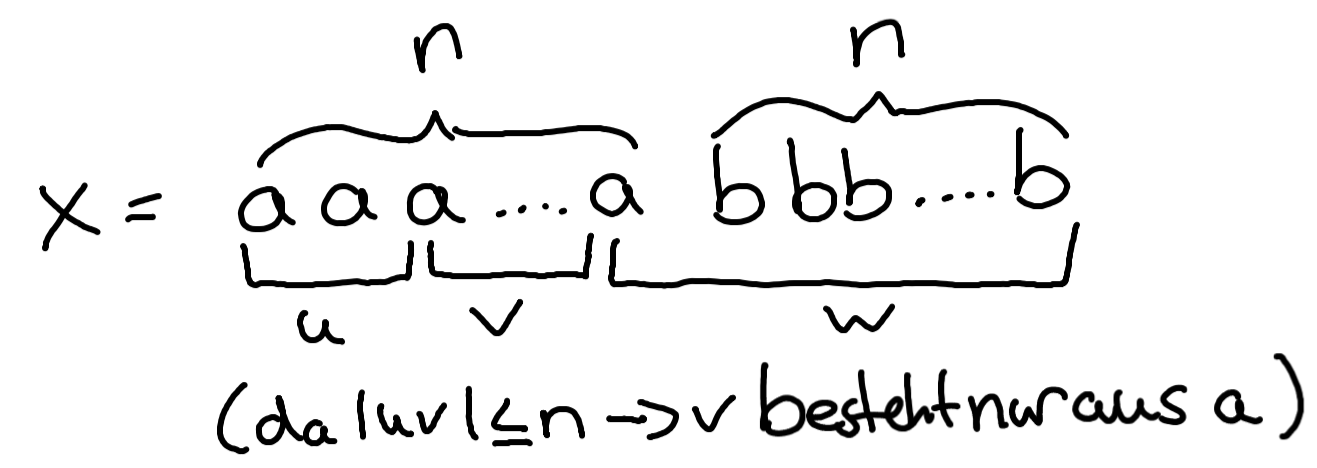
\includegraphics[width=8cm]{pump1}
			\end{center}
		\end{itemize}	


\item {\large \textbf{Pumping Lemma(kontextfrei) - Anwendung}}
	\begin{itemize}
	\item Schema zur Widerlegung:
	\item WENN: 
		\begin{itemize}
		\item $\forall n \in \mathbb{N}$ gilt:
		\item $\exists x \in L mit |x| \geq n$:
		\item $\forall$ Zerlegung $x=yuvwz$ mit $uw \neq \epsilon$ und $|uvw| \leq n$
		\item $\exists m \in \mathbb{N}$, sodass $yu^mvw^mz \notin L$
		\end{itemize}
	\item DANN: 
		\begin{itemize}
		\item $L$ nicht erkennbar | $L$ ist keine reguläre Sprache
		\end{itemize}
	\item[]
	\item \textbf{Beispiel:}
		\begin{itemize}
		\item $L=\{a^nb^nc^n: n \in \mathbb{N}\}$
		\item Sei $n \in \mathbb{N}$ beliebig:
		\item Wähle $x = a^nb^nc^n$:
		\item Zerlegung ...
		\item Fall 1: uvw hat kein c. $m=2$: $yu^mvw^mz$ hat mehr a/b als c $\Rightarrow$ $yu^mvw^mz \notin L$
		\item Fall 2: uvw hat kein a. $m=2$: $yu^mvw^mz$ hat mehr b/c als a $\Rightarrow$ $yu^mvw^mz \notin L$
		\item (Aufgrund von $|uvw| \leq n$ kann es, sobald es ein c hat, kein a mehr haben)
		\item[$\Rightarrow$] L ist nicht kontextfrei
		\end{itemize}
	\end{itemize}

\pagebreak

\item {\large \textbf{Myhill-Nerode - Anwendung}}
	\begin{itemize}
	\item Satz von Myhill-Nerode:
		\begin{itemize}
		\item $L \in \Sigma^*$ ist erkennbar $\Leftrightarrow$ $\sim_L$ hat endlichen Index
		\end{itemize}
	\item Wortäquivalenz $\sim_L$
		\begin{itemize}
		\item $w \sim_L w'~\Leftrightarrow~ \forall x \in \Sigma^*:~(wx \in L \Leftrightarrow w'x \in L)$
		\item Für $\sim_L$ gelten folgende Eigenschaften:
			\begin{itemize}
			\item[1.] $\sim_L$ ist rechts invariant: $w \sim_L w' \Rightarrow \forall u \in \Sigma^* (wu \sim_L w'u)$
			\item[2.] $L$ ist abgeschlossen unter $\sim_L$: $(w\in L \land w \sim_L w') \Rightarrow w' \in L$
			\item[3.] $L$ ist die Vereinigung aller Äquivalenzklassen von $\sim_L$
			\end{itemize}
		\end{itemize}
	\item Zustandsäquivalenz $\sim_A$
		\begin{itemize}
		\item $w \sim_A w' \Leftrightarrow \hat{\delta}(q_0,w) = \hat{\delta}(q_0,w')$
		\item Für $\sim_A$ gelten folgende Eigenschaften:
			\begin{itemize}
			\item[1.]$\sim_A$ hat endlichen Index, nämlich $index(\sim_A) \geq |Q|$
			\item[2.]$\sim_A$ ist rechts-invariant: $w \sim_A w' \Rightarrow \forall u \in \Sigma^* wu \sim_A w'u$
			\item[3.]$\sim_A$ verfeinert $\sim_L$: $w\sim_A w' \Rightarrow w \sim_L w'$
			\end{itemize}
		\end{itemize}
	\item[]
	\item \textbf{Anwendung}
		\begin{itemize}
		\item Aufzeigen unendlich vieler Äquivalenzklassen 
		\item Beispiel: $L=\{w \in \{a,b\}^* |~w~hat~mehr~b~als~a\}$
		\item $k < n$
		\item $b^n a^k \in L$ (Aufstellen von $b^k$ und $b^n$ und Anhängen des selben Wortes)
		\item $b^n a^k \notin L$ (Eins liegt in L, das andere nicht)
		\item Dementsprechend gilt $\sim_L$ nicht
		\item[$\Rightarrow$] $k$ und $n$ hier beliebig gewählt, dementsprechend beliebig viele Äquivalenzklassen
		\item[$\Rightarrow$] $|\sim_L| = \infty$
		\item[$\Rightarrow$] Sprache nicht regulär
		\end{itemize}
		
	\end{itemize}

\end{itemize}

\pagebreak





{\Large \textbf{Algorithmen / Rechenmuster}} 



\begin{itemize}

\item {\large \textbf{Produktautomat Durchschnitt $\cap$ und Schnitt $\cup$}}
	\begin{itemize}
	
	\item[]
		\begin{minipage}{0.4\textwidth}
				\begin{figure}[H]
				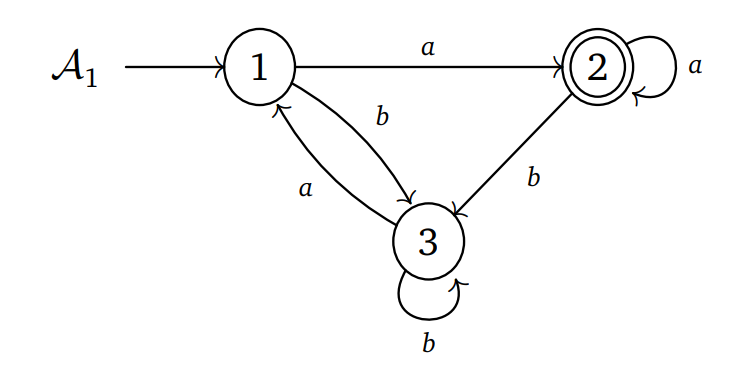
\includegraphics[height=3cm]{durchschnitt1}
				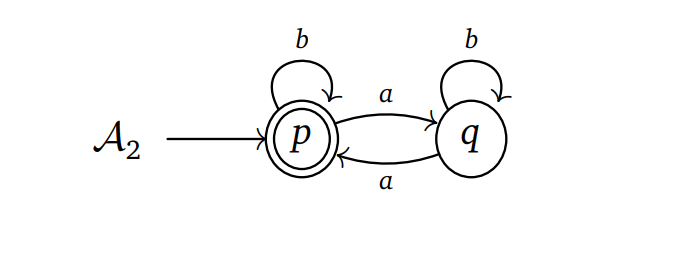
\includegraphics[height=3cm]{durchschnitt3}
				\end{figure}
			\end{minipage}
			\begin{minipage}[t]{0.4\textwidth}
				\vspace{-3cm}
				\begin{figure}[H]
				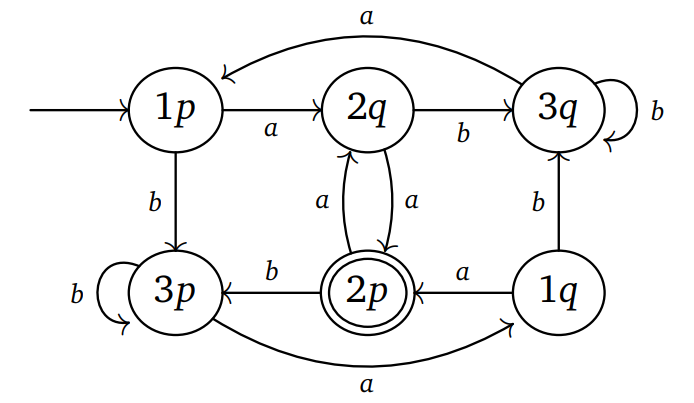
\includegraphics[height=4.5cm]{durchschnitt2}
				\end{figure}
			\end{minipage}
	\item 1. Beide Startzustände zu 1p zusammenfassen
	\item 2. Von dort aus neue Zustände bilden, die man z.B. mit a erreicht
	\item Bsp: $1 \rightarrow^a 2$ und $p \rightarrow^a q$ $\Rightarrow$ 2q
	\item 3. Fortfahren bis alle Zustände abgedeckt sind
	\item \textbf{Akzeptierende Zustände}
		\begin{itemize}
		\item Bei $\cup$: Alle Zustände, die zu mindestens einem Teil aus altem akzeptierenden Zustand bestehen
		\item Bei $\cap$: Alle Zustände, die zu beiden Teilen aus alten akzeptierenden Zuständen bestehen
		\end{itemize}
	
	\end{itemize}
	
\item {\large \textbf{Konkatenations-Automat $\cdot$}}
	\begin{itemize}
	
	\item[]
		\begin{center}
		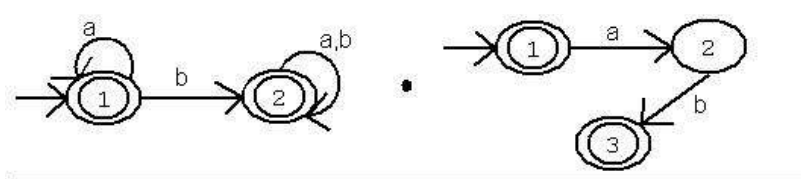
\includegraphics[width=12cm]{konkat1}
		\end{center}			
	
	\item[]
		\begin{center}
		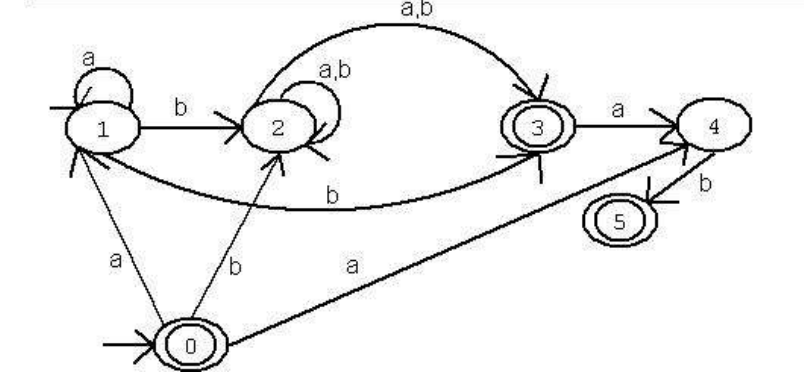
\includegraphics[width=12cm]{konkat2}
		\end{center}	
	
	\item Konkatenation durch Aneinanderhängen zweier Automaten
	\item Für jede Transition des ersten Automaten in dessen Endzustand:
		\begin{itemize}
		\item[$\Rightarrow$] Einbauen einer Transition in den Anfangszustand des anderen Automaten
		\item[$\Rightarrow$] Dies gilt insbesondere auch für Schleifen, die die vom akzep. Zustand auf sich selbst zeigen
		\end{itemize}
	\item \textbf{Akzeptierende Zustände:} nur die des zweiten Automaten
	\item \textbf{Achtung:} Falls erster Automat $\epsilon$ akzeptiert:
		\begin{itemize}
		\item[$\Rightarrow$] Einführen eines extra Startzustands, der alle Transitionen beider Startzustände besitzt
		\item[$\Rightarrow$] Falls beide Automaten $\epsilon$ akzeptieren  $\rightarrow$ neuer Startzustand akzeptierend 
		\end{itemize}
		
	\end{itemize}
	
\pagebreak
	
\item {\large \textbf{Sternautomat * (NFA)}}
	\begin{itemize}
	
	\item Stern-Sprache der aktuellen Sprache	
	
	\item[]
		\begin{minipage}{0.45\textwidth}
				\begin{figure}[H]
				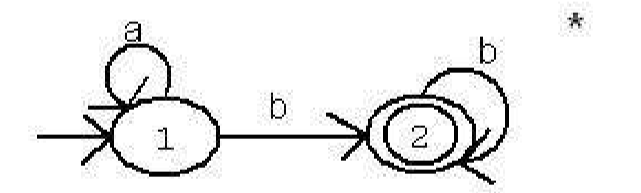
\includegraphics[height=2.5cm]{stern1}
				\end{figure}
			\end{minipage}
			\begin{minipage}[t]{0.45\textwidth}
				\vspace{-1.75cm}
				\begin{figure}[H]
				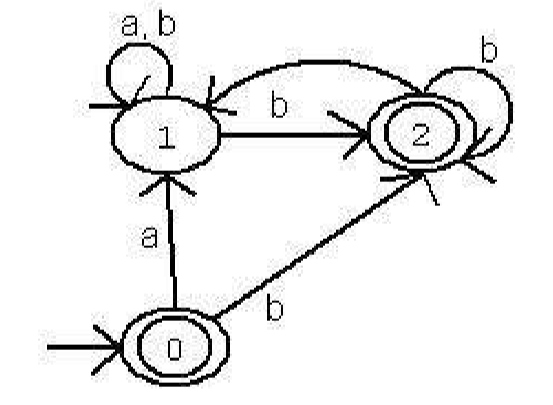
\includegraphics[height=4.5cm]{stern2}
				\end{figure}
			\end{minipage}
	
	\item 1. Einbauen eines neuen akzeptierenden Startzustands
	\item 2. Neuer Startzustand enthält alle Transitionen des alten Starts
	\item 3. Lenkung aller Transitionen, die auf akzep. Zustand zeigen auf den alten Start (oder neuer Start)
	\item (auch Selbstschleifen)
	
	\end{itemize}
	
	
\item {\large \textbf{Komplementbildung eines Automaten $\bar{L}$}}
	\begin{itemize}
	\item Wechsel der akzeptierenden und nicht akzeptierenden Zustände
	\end{itemize}
		
		
\item {\large \textbf{Potenzmengenautomat (NFA $\rightarrow$ DFA)}}
	\begin{itemize}
	\item Jede Zustandsmenge simuliert in welchen Zuständen sich der NFA befinden könnte
	\item 1. Erstellen einer Tabelle und Start bei Anfangszustand \{0\}
	\item 2. Notieren aller Zustände, die der Startzustand mithilfe einer Transition erreicht
	\item 3. Erstellen eines neuen Zeileneintrags mit dieser Menge an Zuständen
	\item 4. Durchführung bis alle Zustände abgedeckt sind
	\item \textbf{Akzeptierende Zustände:} Akzeptiert, falls einer der Zustände in der Menge akzeptierend ist
	\item[]
		\begin{minipage}{0.55\textwidth}
				\begin{figure}[H]
				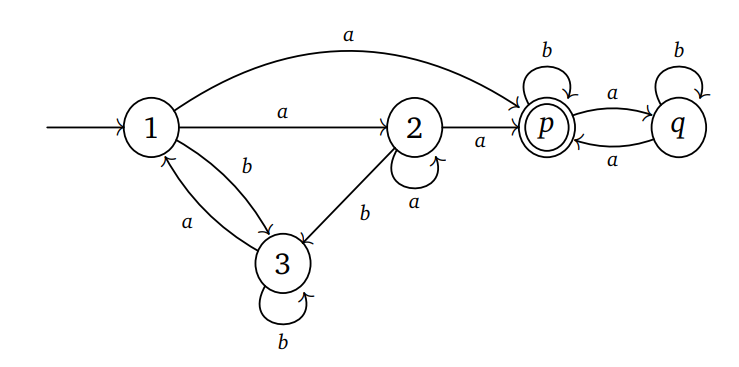
\includegraphics[height=4.5cm]{potenz1}
				\end{figure}
			\end{minipage}
			\begin{minipage}[t]{0.35\textwidth}
				\vspace{-2.25cm}
				\begin{figure}[H]
				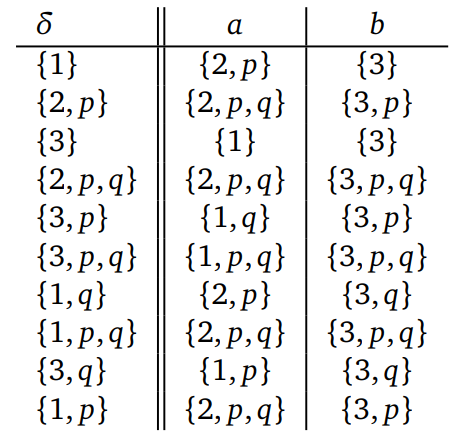
\includegraphics[height=5cm]{potenz2}
				\end{figure}
			\end{minipage}
	\item \textbf{Hier:} Links: NFA    Rechts: Tabelle zu DFA
	\item Beispiel hier: Startzustand führt mit $a$ zu $2$ und $p$ deswegen neuer Zustand mit $\{2,p\}$	
	\item Tipp: Vielleicht hilfreich Transitionstabelle für Quellautomaten zu machen (Ablesefehler)
	
	\end{itemize}

\pagebreak

\item {\large \textbf{Satz von Kleene (Automat $\rightarrow$ regulärer Ausdruck)}}
	\begin{itemize}
	\item Durchführen von k Iterationschritten zum Erhalten des regulären Ausdrucks
	\item k = Anzahl der Zustände
	\item Rekursionsformel: $a^{k+1}_{l,m} = a^k_{l,m} + a^k_{l,k+1}(a^k_{k+1,k+1})^*a^k_{k+1,m}$
	\item[]
	\item \textbf{Durchführung}
		\begin{itemize}		
		\item 1. Aufstellen von $a^0_{l,m}$ mithilfe der Formel:
		\item[]
			\begin{center}
			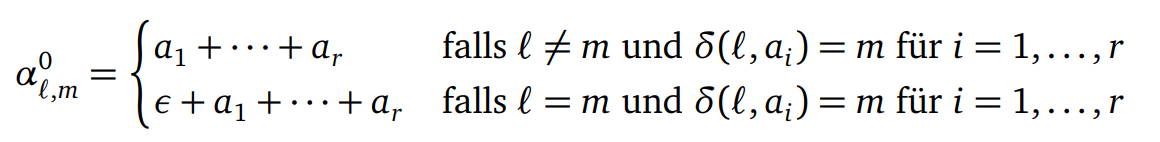
\includegraphics[height=1.5cm]{kleene1}
			\end{center}
		\item 2. Anwendung der Rekursionsformel zur Erstellung von $a^k_{l,m}$
		\item 3. Durchführung bis $a^{k-1}_{l,m}$
		\item 4. Danach Durchführung für die ''akzeptierende Zelle'' um regulären Ausdruck zu erhalten
	\end{itemize}
	\item[]
	\item Tipps: (in k-ter Tabelle)
		\begin{itemize}
		\item $a^k_{l,m}$:			entspricht Werten in vorheriger Tabelle an selber Stelle
		\item $a^k_{l,k+1}$:		entspricht jeweils den Werten der k-ten Spalte in vorheriger Tabelle
		\item $(a^k_{k+1,k+1})^*$: ist für die ganze Tabelle der selbe Wert (k-te Zeile, k-te Spalte)
		\item $a^k_{k+1,m}$:		entspricht jeweils den Werten der k-ten Zeile in vorheriger Tabelle
		\end{itemize}
	\item \textbf{Beispiel im Anhang}
	
	\end{itemize}
		
		
\item {\large \textbf{Minimierung eines Automaten}}
	\begin{itemize}
	\item 1. Start bei $\sim_0$: Einteilung der Zustände in Akzeptierend und Nicht-Akzeptierend
	\item 2. Eintragen in Tabelle mit Klassen $\rightarrow$ Transitionen enden in Klassen
	\item 3. Aufteilung einer Klasse in Unterklasse, falls Elemente unterschiedliche Transitionen haben
	\item 4. Durchführung für $\sim_{i+1}$, bis jedes Element in jeder Klasse die selbe Transition hat
	\item 5. Aufzeichnen des neuen Automaten mit Klassen als Zustände
	\item \textbf{Akzeptierende Klasse/Zustände}: Klasse, die akzeptierende Zustände enthält
	\item[]
	\item[]
		\begin{center}
		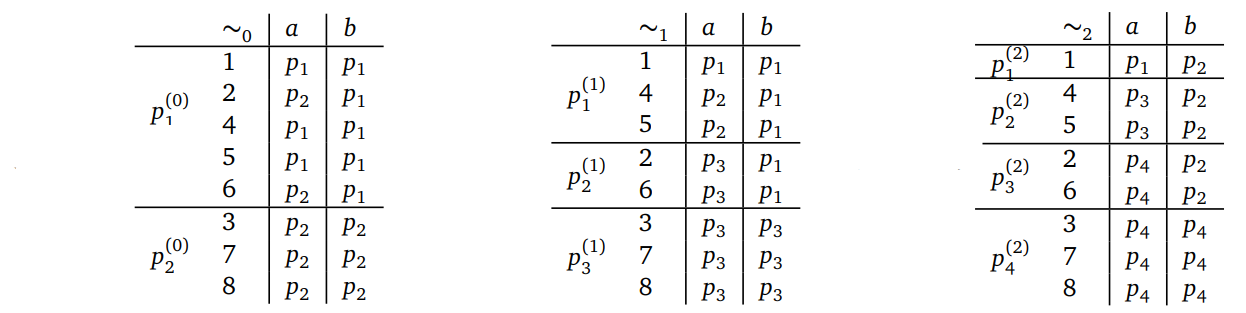
\includegraphics[height=4cm]{minautomatbsp}
		\end{center}
	\end{itemize}			

\pagebreak


\item {\large \textbf{Umformung kontextfreier Grammatik in Chomsky-Normalform}}
	\begin{itemize}
	\item \textbf{Bedingung:} Alle Produktionen in Form: $X \rightarrow YZ$ oder $A \rightarrow a$
	\item[]
	\item \textbf{Durchführung}
		\begin{itemize}
		\item 1. Eliminiere $\epsilon$-Produktionen	
			\begin{itemize}
			\item 1.1 Aufstellen einer Nicht-Terminal-Menge, die zu $\epsilon$-Produktionen führt
			\item 1.2 Ersetzen durch alle möglichen Kombinationen ohne $\epsilon$ an Stellen aus Menge
			\item[]
				\begin{minipage}{0.4\textwidth}
					\begin{figure}[H]
					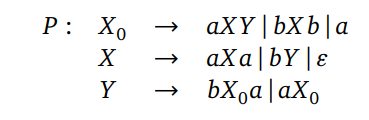
\includegraphics[height=1.5cm]{epsi1}
					\end{figure}
				\end{minipage}
				\begin{minipage}[t]{0.4\textwidth}
					\vspace{-1cm}
					\begin{figure}[H]
					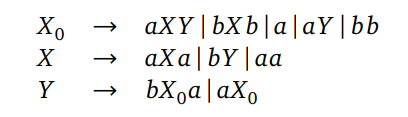
\includegraphics[height=1.5cm]{epsi2}
					\end{figure}
				\end{minipage}
			\end{itemize}
		\item 2. Variablen für Terminale einfügen ($A \rightarrow a, B \rightarrow B$)
		\item 3. Kettenproduktionen eliminieren ($X \rightarrow Y$)
		\item 4. Eliminiere $X \rightarrow X_0,..,X_k$ mit $k \geq 3$ (Mehr als 2 Variablen aufteilen)
		\item Aus $A \rightarrow ABC$ wird $A \rightarrow AD$ und $D \rightarrow BC$
		\end{itemize}
		
	\item \textbf{Beispiel im Anhang}
	\end{itemize}


\item {\large \textbf{CYK Algorithmus}}
	\begin{itemize}
	\item Bestimmung des Wortproblems für kontextfreie Grammatiken in CNF
	\item[]
	\item \textbf{Durchführung}
		\begin{itemize}
		\item 1. Aufstellen einer Tabelle (Größe nxn (n = Wortlänge)
		\item 2. Eintragen der Integranden für einzelne Buchstaben in oberste Zeile
		\item 3. Ausfüllen der Tabelle (guckt euch 'n Video an)
		\item 4. Falls das Startsymbol in der letzten Zeile entsteht $\rightarrow$ Wort wird durch Grammatik erkannt
		\end{itemize}
	\item Ableitungsbaum ausgehend von S erstellen, falls benötigt
	\end{itemize}


\item {\large \textbf{Reguläre Grammatiken $\Leftrightarrow$ Automaten}}
	\begin{itemize}
	\item Ziemlich selbstverständlich anhand Beispielen
	\item[]
				\begin{minipage}{0.4\textwidth}
					\begin{figure}[H]
					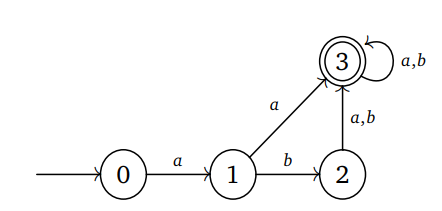
\includegraphics[height=2cm]{reggra1}
					\end{figure}
				\end{minipage}
				\begin{minipage}[t]{0.4\textwidth}
					\vspace{-1cm}
					\begin{figure}[H]
					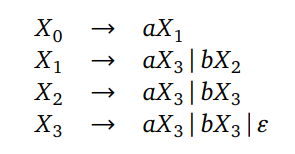
\includegraphics[height=2cm]{reggra2}
					\end{figure}
				\end{minipage}
	
	\item[]
				\begin{minipage}{0.4\textwidth}
					\begin{figure}[H]
					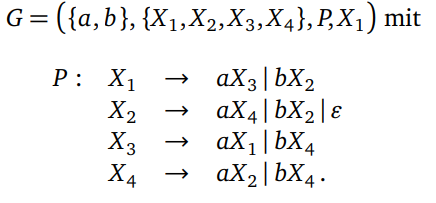
\includegraphics[height=2.5cm]{reggra3}
					\end{figure}
				\end{minipage}
				\begin{minipage}[t]{0.4\textwidth}
					\vspace{-1.25cm}
					\begin{figure}[H]
					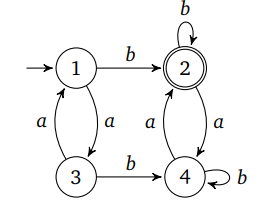
\includegraphics[height=2cm]{reggra4}
					\end{figure}
				\end{minipage}
	\end{itemize}

\end{itemize}

\pagebreak



{\Large \textbf{Automatenbeispiele}}

\begin{itemize}

\item L: Wörter, in denen 100 als Teilwort vorkommt
	\begin{itemize}
	\item $a = (0+1)^*100(0+1)^*$
	\item[]
		\begin{center}
		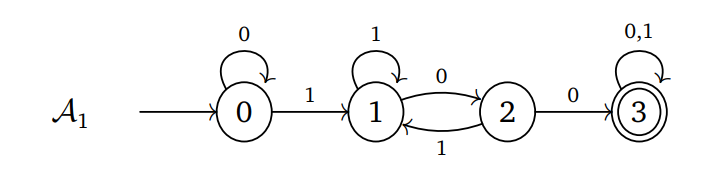
\includegraphics[width=8cm]{auto1}
		\end{center}	
	\end{itemize}

\item L: Wörter mit gerader Anzahl von 1
	\begin{itemize}
	\item $a=(0+10^*1)^*$
	\item[]
		\begin{center}
		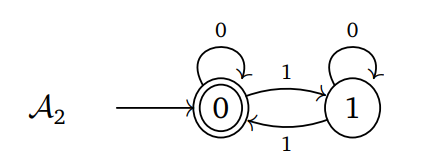
\includegraphics[width=8cm]{auto2}
		\end{center}	
	\end{itemize}
	
\item L: Wörter mit gerader Anzahl von 1 und genau zweimal 0
	\begin{itemize}
	\item Mit $\alpha = 1(11)^* und \beta=(11)^*$
	\item $a = \alpha0\alpha0\beta + \alpha0\beta0\alpha + \beta0\alpha0\alpha + \beta0\beta0\beta$
	\item[]
		\begin{center}
		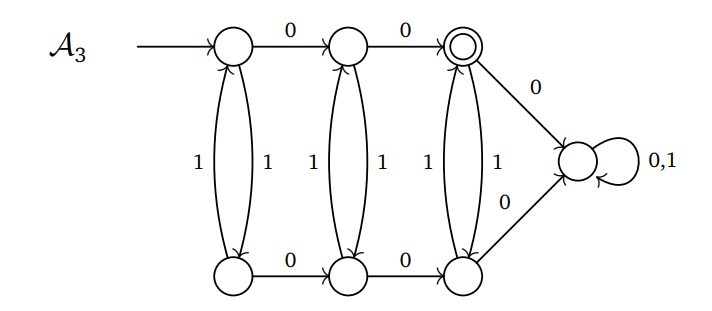
\includegraphics[width=8cm]{auto3}
		\end{center}	
	\end{itemize}
	
\item L: Wörter von ungerader Länge mit genau zwei 1
	\begin{itemize}
	\item[]
		\begin{center}
		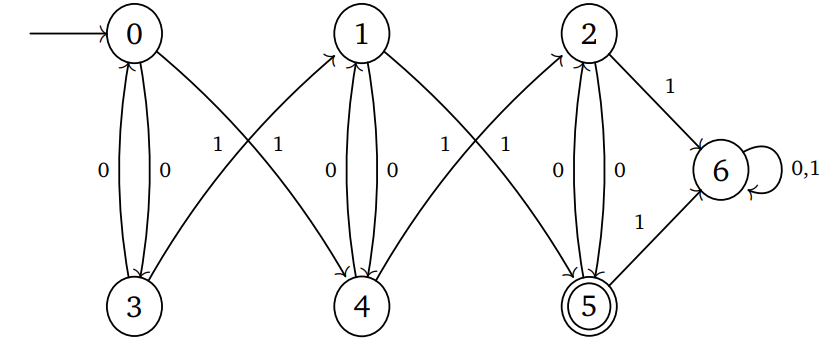
\includegraphics[width=8cm]{auto4}
		\end{center}	
	\end{itemize}
	
\item L: Wörter, die 01 und 10 als (nicht notwendigerweise disjunkte) Teilwörter enthalten
	\begin{itemize}
	\item[]
		\begin{center}
		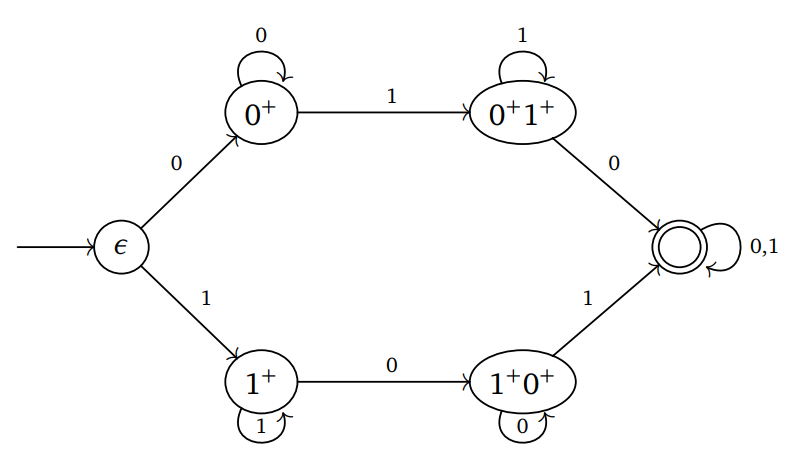
\includegraphics[width=8cm]{auto5}
		\end{center}	
	\end{itemize}

\item L: Wörter, in denen alle 1-Blöcke eine Länge der Form $2n+3$ haben
	\begin{itemize}
	\item[]
		\begin{center}
		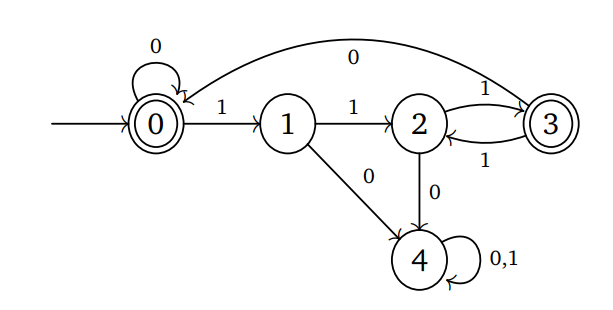
\includegraphics[width=8cm]{auto6}
		\end{center}	
	\end{itemize}
	
\item L = $L(((a+b)(c+d))^*)$
	\begin{itemize}
	\item[]
		\begin{center}
		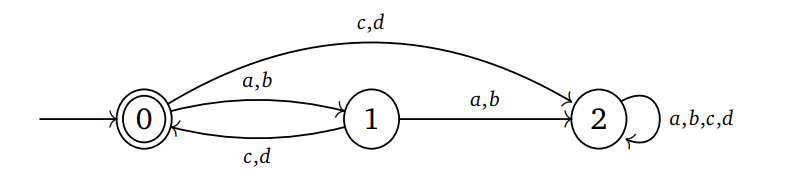
\includegraphics[width=8cm]{auto7}
		\end{center}	
	\end{itemize}

\end{itemize}

\pagebreak

{\Large \textbf{Sprachen $\Rightarrow$ Grammatik}
\begin{itemize}

\item $L((bc + a)^*aba(ac+b)^*)$
\begin{center}
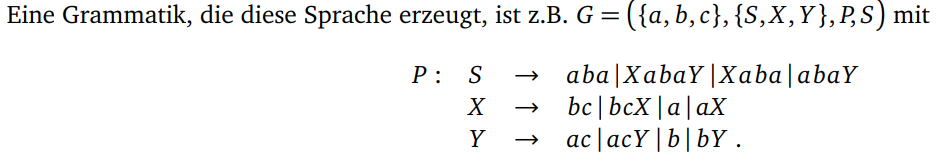
\includegraphics[width=12cm]{gram1}
\end{center}

\item $L=\{ucw \in \{a,b,c\}^* | u,w \in {a,b,c}^*, |u_b| = |w_b|\}$
\begin{center}
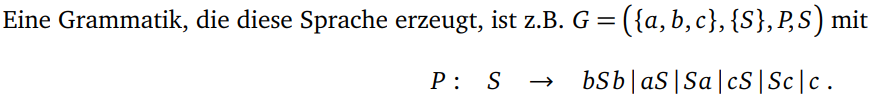
\includegraphics[width=12cm]{gram2}
\end{center}

\item[]
\begin{center}
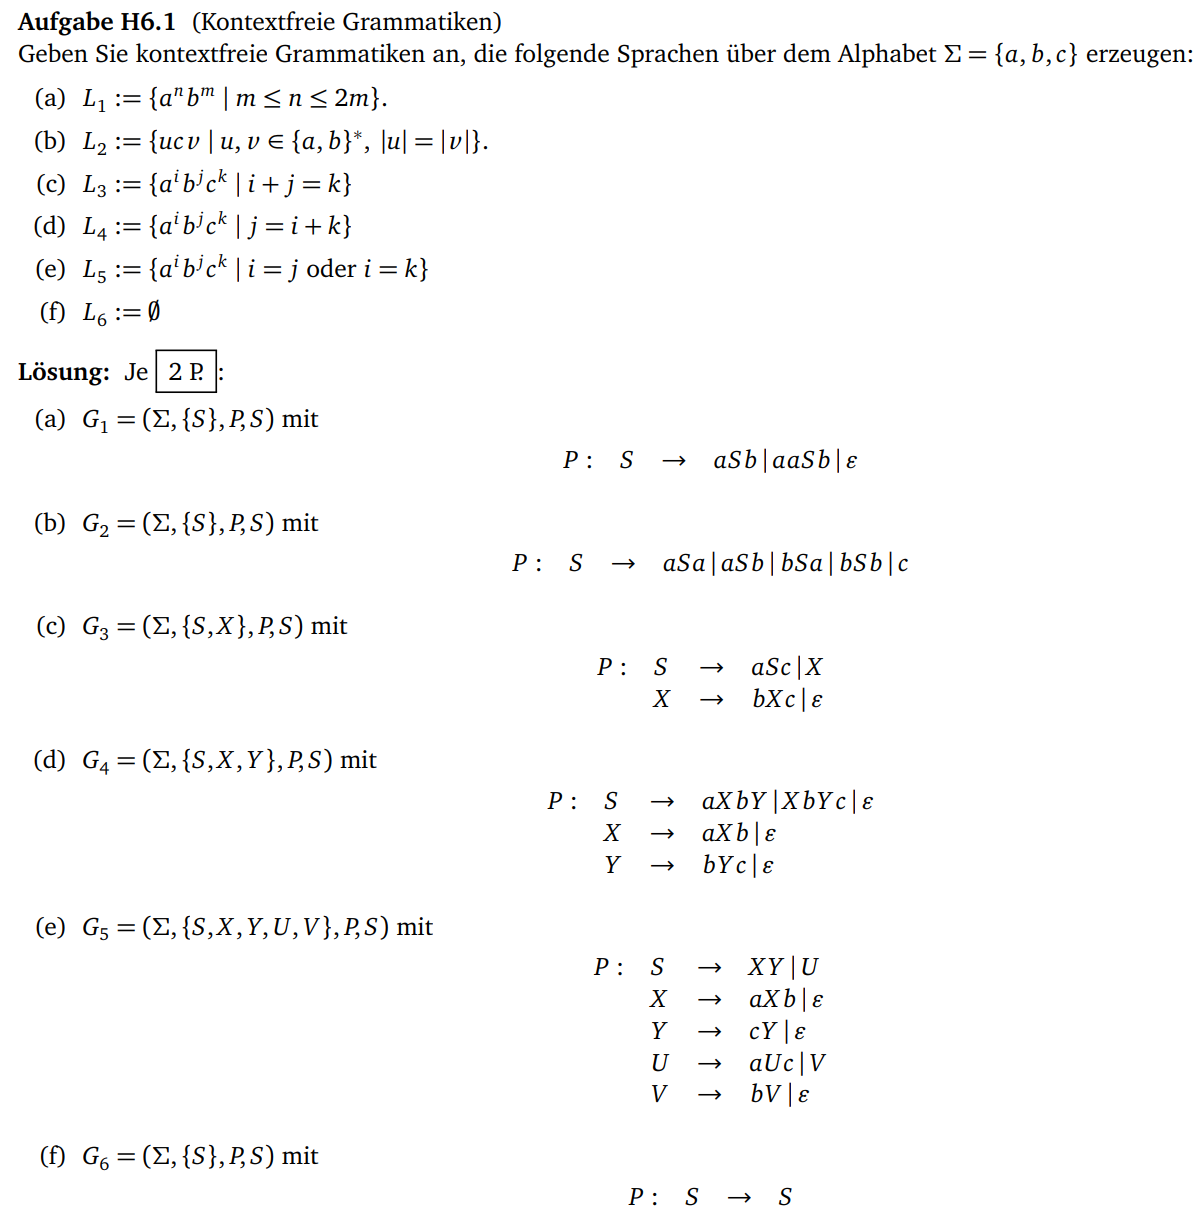
\includegraphics[scale=1]{gram3}
\end{center}

\end{itemize}

\pagebreak

{\Large \textbf{Satz von Kleene - Beispiel}}

\begin{center}
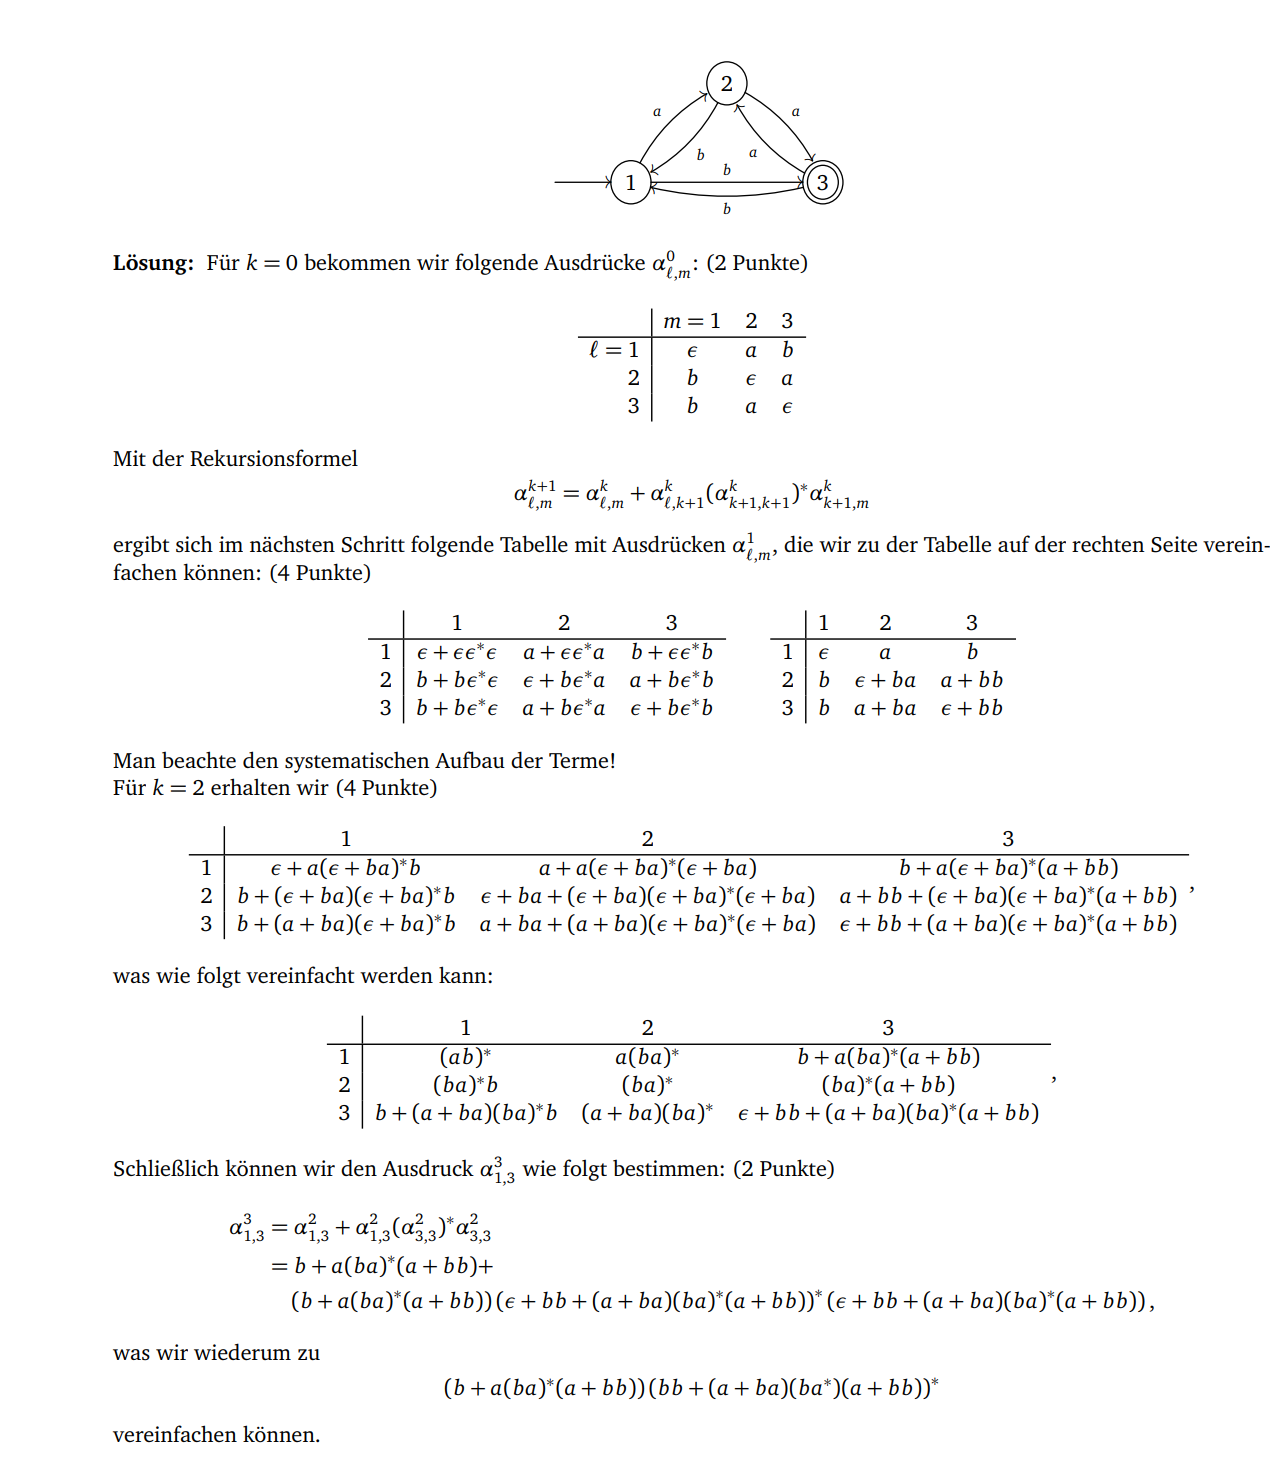
\includegraphics[scale=1]{kleenebsp}
\end{center}

\pagebreak

{\Large \textbf{Chomsky-Normalform - Beispiel}

\begin{center}
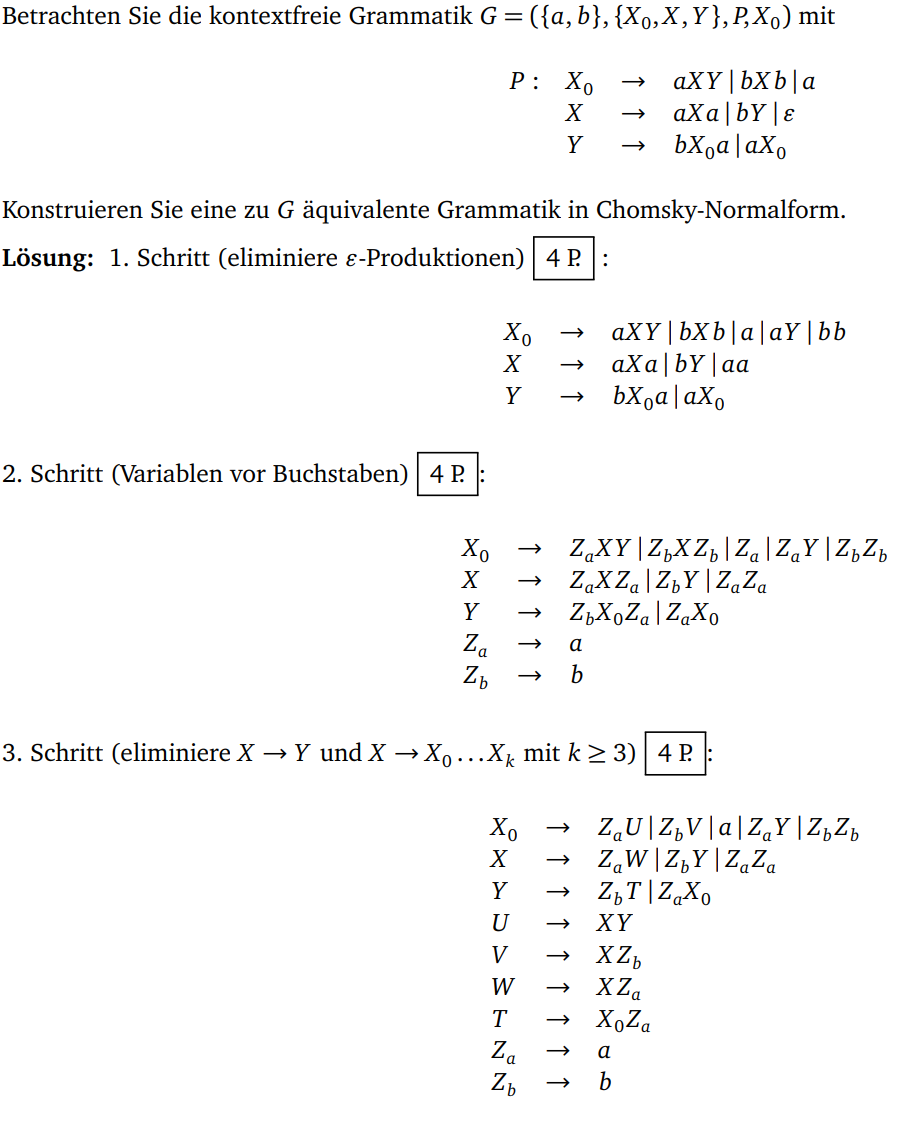
\includegraphics[scale=1]{chomskybsp}
\end{center}

\pagebreak

{\Large \textbf{Quizfragen}}

\begin{center}
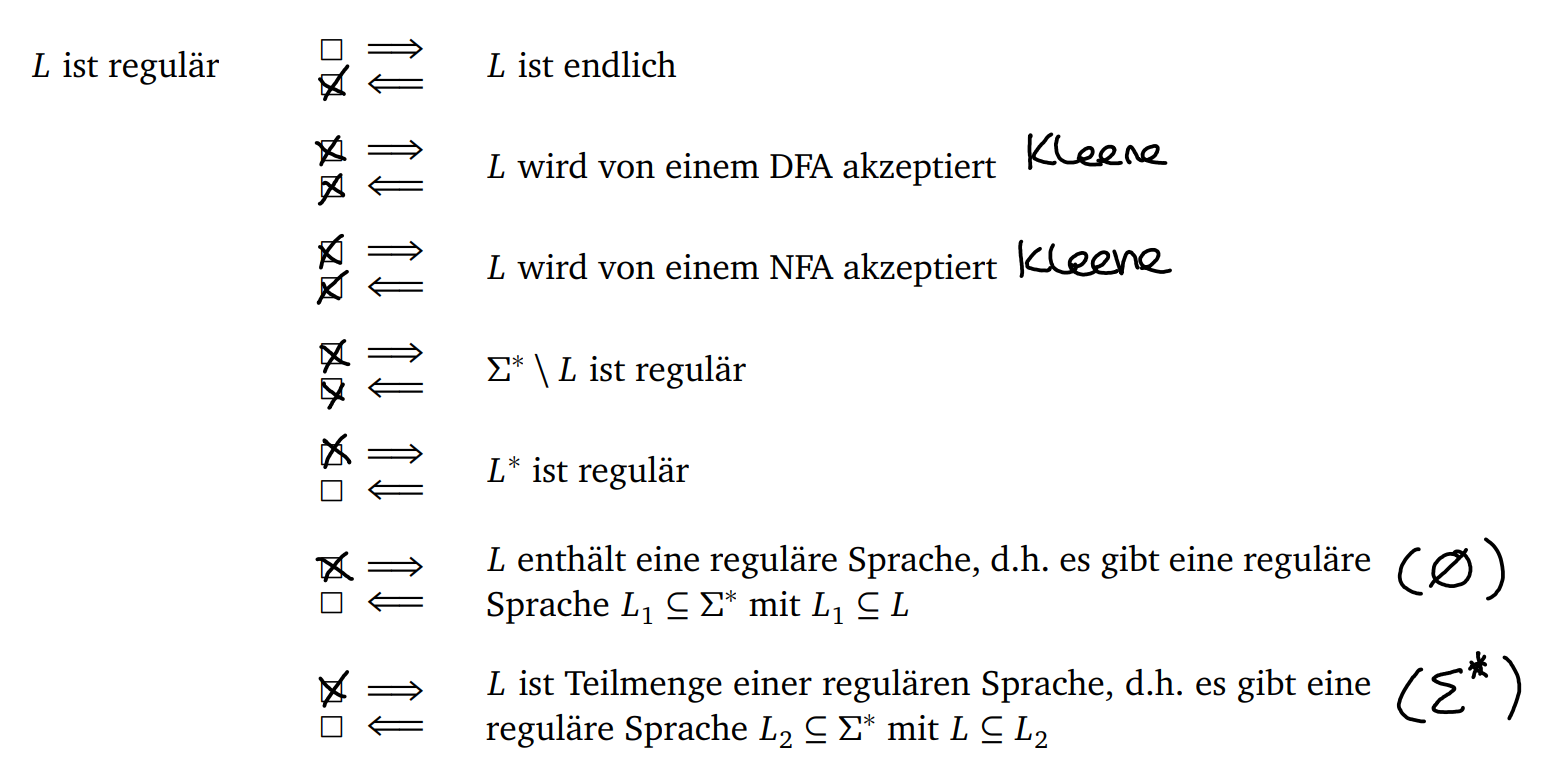
\includegraphics[width=12cm]{quiz1}
\end{center}

\begin{center}
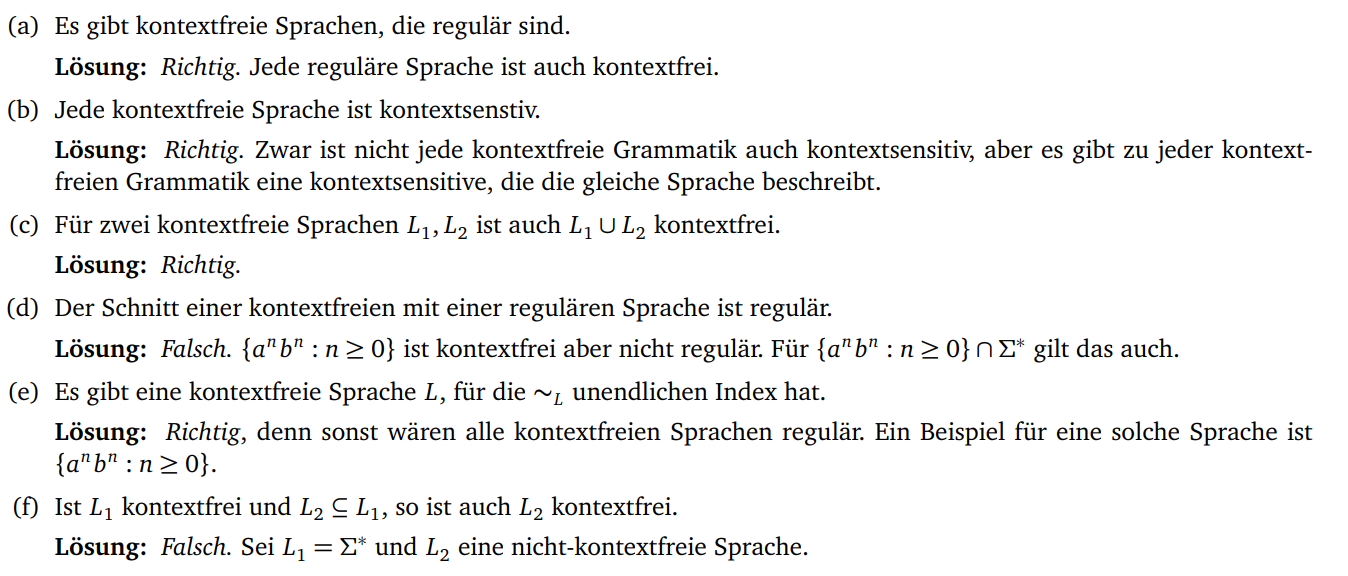
\includegraphics[width=15cm]{quiz2}
\end{center}


{\Large \textbf{Erstellung Kellerautomat aus Grammatik}}

\begin{center}
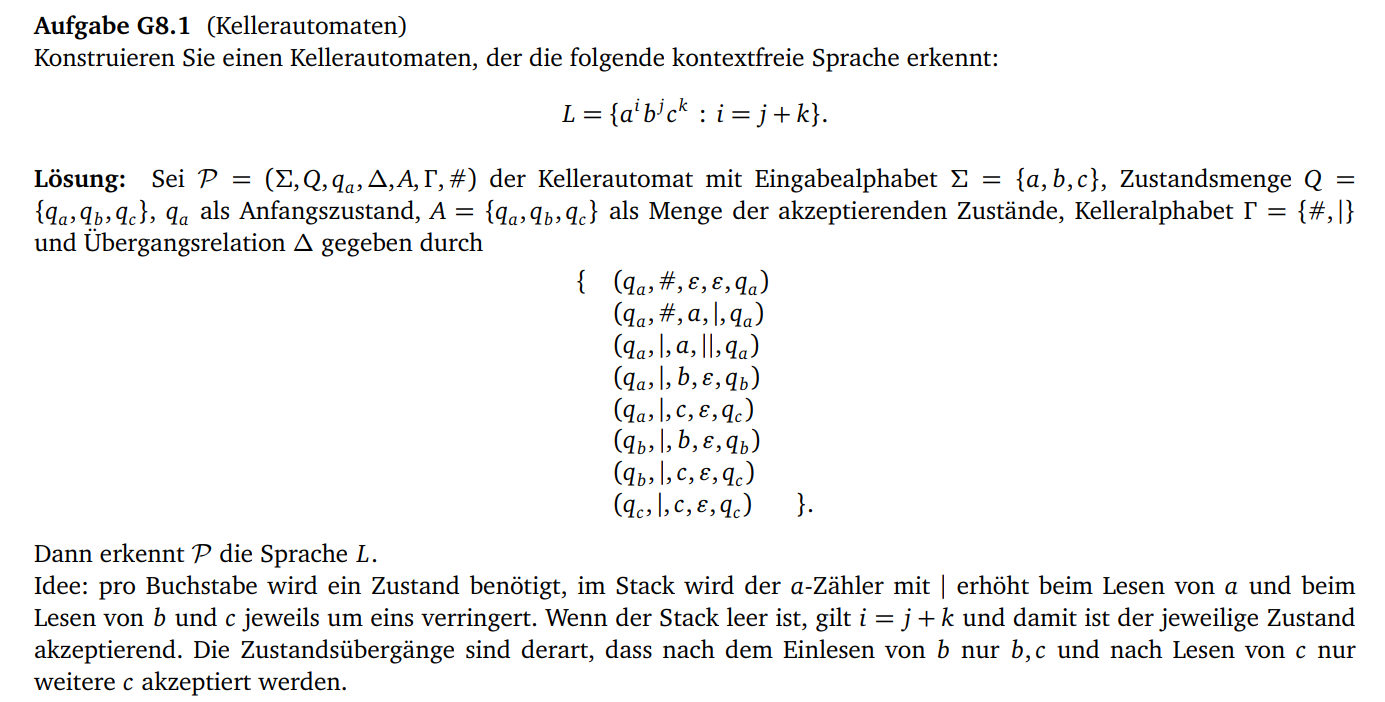
\includegraphics[scale=1]{keller1}
\end{center}



\end{document}